\chapter{Properties of an n-channel enhancement MOSFET}


\section{Objectives}
\begin{itemize}
    \item To find the voltage-current characteristics of a n-channel enhancement MOSFET
    \item To evaluate different operation modes of a n-channel enhancement MOSFET
\end{itemize}

\section{Materials}
\begin{itemize}
    \item Breadboard
    \item Capacitors
    \item DC power supply
    \item Digital Multi-Meter
    \item \hyperref[2N7000_1]{MOSFET (2N7000)}
    \item Resistors
\end{itemize}

\section{Introduction}
    \subsection{Circuit Diagram}
    \begin{figure}[h]
        \centering
        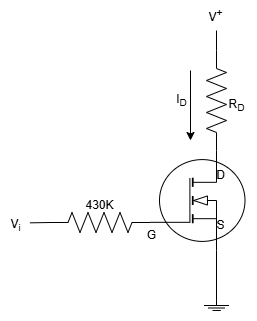
\includegraphics[width=0.65\linewidth]{Lab08/Lab8.drawio.png}
        \caption{Circuit Diagram}
        \label{l8f}
    \end{figure}
    \FloatBarrier

\section{Detailed Procedures}
    \subsection{Analyzation}


    \subsection{Procedures}

    
\section{Discussion}


\section{Conclusion}
